%---------------------------------------------------------------------------%
%->> Main content
%---------------------------------------------------------------------------%
\section{学位论文进展情况,存在的问题,已取得阶段性成果}
\subsection{LATA-V动态翻译器的设计和实现}
在翻译器LATA的基础上,我实现了龙芯平台上ARM64的动态翻译器LATA-V;相比于前者,LATA-V进一步完善指令翻译,支持了ARM的向量和浮点指令到龙架构的翻译;在指令翻译的过程中,引入指令随机测试框架,能够根据指令pattern和指令数量生成测试案例,支持单指令的随机测试。同时,为了方便翻译器在运行大型应用时的调试,设计并实现了基于 QEMU 的调试框架。目前,LATA-V的总体框架已经基本完成,实现了约500条ARM架构指令的翻译,其中浮点和向量指令约为200条左右,LATA-V已能够正确运行ARM64的SPEC CPU2006基准测试程序,包括所有的定点和浮点子项;随机指令测试框架也已经能够正常运行,能够在指令翻译和性能优化过程中发现错误的翻译;调试框架的总体功能也基本实现,完成了LATA-V和QEMU的寄存器状态的对齐,支持指令粒度和基本块粒度的检查点的设置,能够定位不同负载中指令随机组合的翻译错误,弥补随机指令测试框架只能进行单指令测试的不足。
\subsubsection{LATA-V总体框架}
LATA-V的总体框架主要由3个部分组成,包括代码查找,代码执行和指令翻译等模块,主要的流程如图\ref{fig:LATA-V}所示。

\begin{figure}[!htbp]
    \centering
    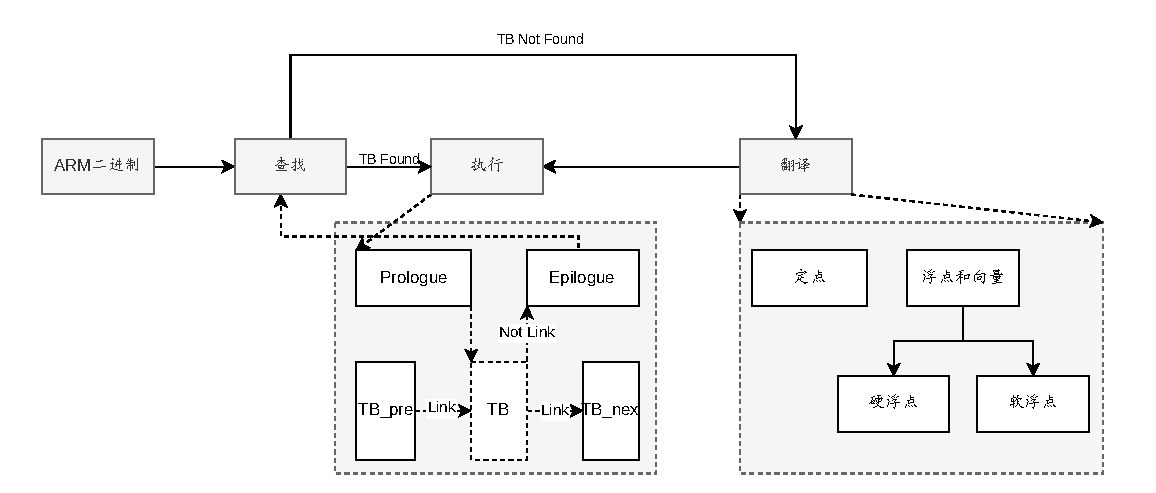
\includegraphics[width=1\textwidth]{LATA-V}
    \bicaption{\enspace LATA-V动态翻译器}{\enspace LATA-V Dynamic Translator}
    \label{fig:LATA-V}
\end{figure}
\textbf{代码查找:}在LATA-V翻译器中,大部分代码块会被重复执行;为了减少代码块的重复翻译,翻译好的代码块通常会被存储到代码缓存中;在执行翻译代码前,翻译器会先根据下一个代码块的PC查找代码缓存,如果代码块在代码缓存中命中,翻译器会进入执行阶段;如果没有命中,翻译器则会进入指令翻译阶段。

\textbf{指令翻译:}在指令翻译阶段,LATA-V翻译器会以基本块为粒度进行指令翻译。LATA-V中基本块的划分受多种条件的约束:一是受基本块内指令的数量的影响,一般来说,基本块中指令的数量是翻译器的可以设置的一个参数,例如可以设置基本块的指令数量为1,从而实现指令的单步执行,LATA-V也不例外;同时,由于翻译资源的限制,基本块内的指令数量会有一个上限值,该上限值的大小和翻译器的指令集架构相关,在LATA-V中该值为512。二是基本块的划分受指令类型的影响,在LATA-V中,基本块以跳转指令或者系统调用指令为结束的标志,这是因为在二进制翻译中,基本块通常定义为一个具有单一入口和单一出口的连续指令序列,其内部不包含控制流的中断。在划分基本块的过程中,LATA-V会对二进制代码进行解码,提取出操作码以及其他相关信息(如操作数、寻址模式等),解码后的操作码会作为键,在预先构建的映射表中查找相应的翻译函数,该映射表在LATA-V中是一个巨型的switch-case结构。查找到对应的翻译函数后,翻译器调用该函数将ARM架构的指令直接转换为Loongarch架构的伪指令表示,同时进行必要的优化和重定位。重定位阶段,翻译器会将龙架构的伪指令转换为汇编源代码,之后汇编模块将由汇编源码生成的二进制代码装入代码缓存中。如果映射表中未找到匹配的操作码,LATA-V通常会调用一个默认的错误处理函数或支持的补充模块,以处理特殊或未预见的指令。指令翻译根据指令类型的不同,可以分为定点指令,浮点和向量指令以及特殊指令的翻译。定点指令的翻译是LATA-V中比较容易的部分,唯一需要注意的是:由于ARM架构和Loongarch架构对于高位拓展的处理不同(ARM架构高位清零,Loongarch架构高位符号拓展),在使用龙架构的指令模拟32位的ARM架构指令时,需要对相应的结果进行高位清零操作。浮点和向量指令在翻译阶段有两种处理方式:一是硬浮点的方式,直接通过对应的龙架构的向量和浮点指令进行翻译,包括向量拓展指令(LSX)和高级向量拓展指令(LASX),分别支持ARM架构128位和256位向量和浮点指令的翻译;二是软浮点的方式,软浮点的存在是为了解决硬件浮点支持不足时对浮点运算的需求,LATA-V会将一些难以通过Loongarch浮点指令拓展的直接翻译的ARM指令映射到helper函数,这些函数是在LATA-V内部实现的IEEE 754标准的浮点运算,保证模拟环境中浮点运算的正确性和一致性;软浮点方式翻译的浮点指令的效率通常比较低,所以只针对一些指令频度较低或者实在难以直接翻译的ARM浮点指令才使用软浮点方式进行翻译。对于一些特殊指令,例如系统调用指令或者一些非法指令,LATA-V也是通过helper函数通过将模拟的过程通过高级语言实现,减少翻译的难度,同理这些指令的翻译效率也是较低的,具体效率较低的原因在代码执行部分会有涉及。

\textbf{代码执行:}对于二进制翻译器来说,代码的执行分成3个部分,分别是翻译态,执行态以及翻译器和执行态间的上下文切换。翻译态包括代码查找和指令翻译阶段的代码,执行态则包括代码缓存中的代码以及的helper函数中的代码,而上下文切换部分由两个基本块组成,在图\ref{fig:LATA-V}中由Prologue和Epilogue命表示。Prologure,Epilogue以及翻译好的基本块TB共同组成了代码缓存。翻译好的基本块在代码缓存中只是简单地按顺序放置,如果不做基本块间的链接,每个基本块结束后都需要返回翻译态中查找下一个基本块块的入口地址,这样会带来巨大的上下文切换开销。通过链接,当一个基本块的末尾遇到跳转指令(如无条件跳转、条件跳转、调用等)时,LATA-V会尝试解析跳转地址:如果目标基本块已经被翻译并存在于代码缓存中,则LATA-V会将当前基本块末尾的跳转指令直接修补为跳转到目标块的入口地址。如果目标块尚未翻译,则可以先使用一个跳转桩(trampoline)或者占位符,待目标块翻译完成后,再进行修补。上下文切换的高开销是导致翻译器效率低下的关键因素之一,同时也是helper函数性能较低的主要原因。

\subsubsection{随机指令测试框架}
随机指令测试框架主要由2部分组成,分别为随机指令生成器以及验证器;
随机指令生成器是一个生成测试数据块的 Perl 脚本,可以在任意地方执行。验证器是一个运行在目标架构(例如ARM架构)的 Linux 可执行文件。
随机指令测试框架的流程如图\ref{fig:RISU}所示。首先,测试配置文件中定义了待测试的指令格式,包括指令编码,寻址模式以及相关的限制。生成器脚本根据测试配置文件以及用户输入的指令模板和测试数量生成包含随机指令的二进制指令数据,该数据是一条待测试指令和一条非法指令交替排列的,非法指令的用处之后会解释。随后,验证器程序分别在主设备(真实硬件或参考平台,这里使用的是QEMU)和从设备(待测模拟器,这里是LATA-V)上加载并执行该数据,执行过程中每条指令后的寄存器状态都会进行交叉比对。若出现不一致或异常,则记录到日志并输出错误信息;若无异常则继续执行,直至全部指令完成。最终,主设备端会打印寄存器状态及对比的结果,帮助定位并修复模拟器在指令实现或解码上的问题,从而有效验证指令集的正确性与稳定性。

寄存器检查通过为非法指令信号(SIGILL,Signal Illegal Instruction)注册一个例外处理程序来实现,该处理程序可通过其 sigcontext 参数访问寄存器内容;
在 Unix/Linux 系统中,当一个信号被触发时,内核会捕获当时进程的状态信息,并将其保存到一个结构体中,这个结构体通常称为 \texttt{sigcontext}。它包含了当时 CPU 的寄存器值、程序计数器(PC)、栈指针、标志寄存器等关键信息。对于使用 \texttt{SA\_SIGINFO} 标志设置的信号处理程序,处理函数通常会收到一个指向 \texttt{ucontext\_t} 的指针,其中就包含了一个 \texttt{sigcontext}。这样,信号处理程序就可以通过 \texttt{sigcontext} 获取或修改进程在信号发生时的状态,这在调试、错误恢复或捕捉非法指令(如 \texttt{SIGILL})的场景中非常有用。
%load 和 store的比较:
% /* Map writable because we include the memory area for store
% * testing in the image.
% */
% addr = mmap(0, len, PROT_READ | PROT_WRITE | PROT_EXEC,
%            MAP_PRIVATE, fd, 0);
% 这种方法存在一些明显的局限性:

% 状态访问局限:
% 我们假设所有重要状态都位于信号处理程序可访问的寄存器中。这在大多数情况下成立,但无法测试如 ldrexd/strexd 这样复杂的指令。

% 生成器简单:
% 生成器相对简单,只是交替生成指令和“检查寄存器”命令。因此,分支、加载或存储指令无法通过这种方式进行检查(这主要是生成器的限制,而非测试框架本身的缺陷)。

% 错误捕捉范围有限:
% 我们仅能捕捉解码或指令实现中的明显错误,而不会检测到诸如模型代码生成器中对指令过于激进的重新排序等问题。

% 测试范围限制:
% 按设计,我们只能测试用户态可见的指令,而无法测试仅对特权代码可见的指令。

% 另外,还有一些较为偶然的限制:

% 我只测试 ARM 架构。生成器设计较为针对 ARM,虽然测试框架本身(例如也有一个 x86 实现的骨架)不那么依赖平台,但实际只进行了 ARM 测试。
% 目前不比较浮点状态标志,原因在于我确信 qemu 目前还未正确处理这些标志,而且我更关注修复严重错误。
% 目前不支持“记录与重放结果”模式。这一模式本可以让你在 ARM 主机上记录正确结果,然后在缺乏对应原生硬件的情况下测试模型实现。
% 你可以选择静态编译以避免 qemu 测试时需要 ARM chroot 的要求,但这样你就不能使用 gethostbyname(),必须通过 IP 地址指定主机。
\begin{figure}[!htbp]
    \centering
    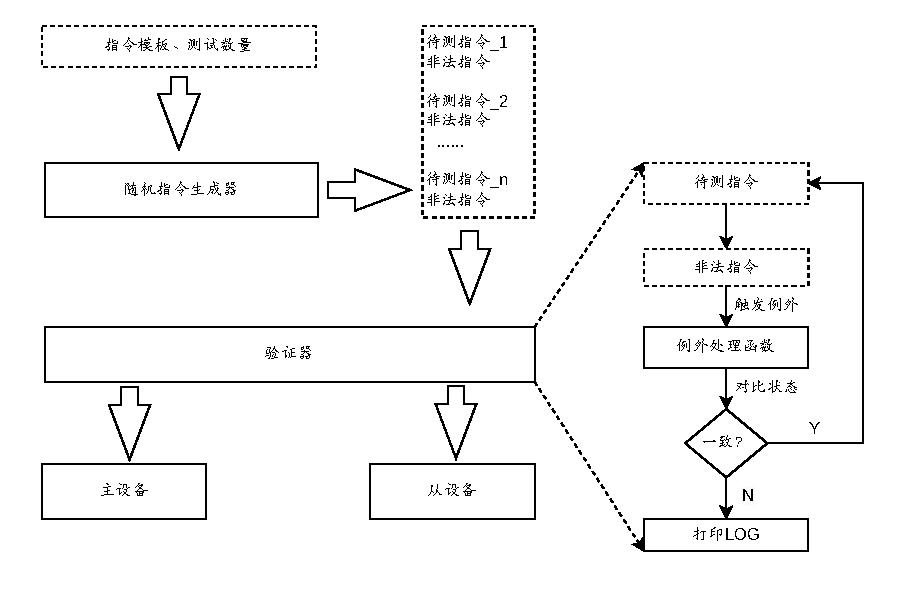
\includegraphics[width=1\textwidth]{RISU}
    \bicaption{\enspace 随机指令测试框架}{\enspace Random Instruction Testing Framework}
    \label{fig:RISU}
\end{figure}

\subsubsection{基于QEMU的调试框架}
调试框架分为顺序模式和二分模式,能够实现指令粒度,基本块粒度的调试。
顺序模式能够精确定位出错的指令或者基本块;二分模式二分查找程序的出错点,能实现快速定位;

\begin{figure}[!htbp]
    \centering
    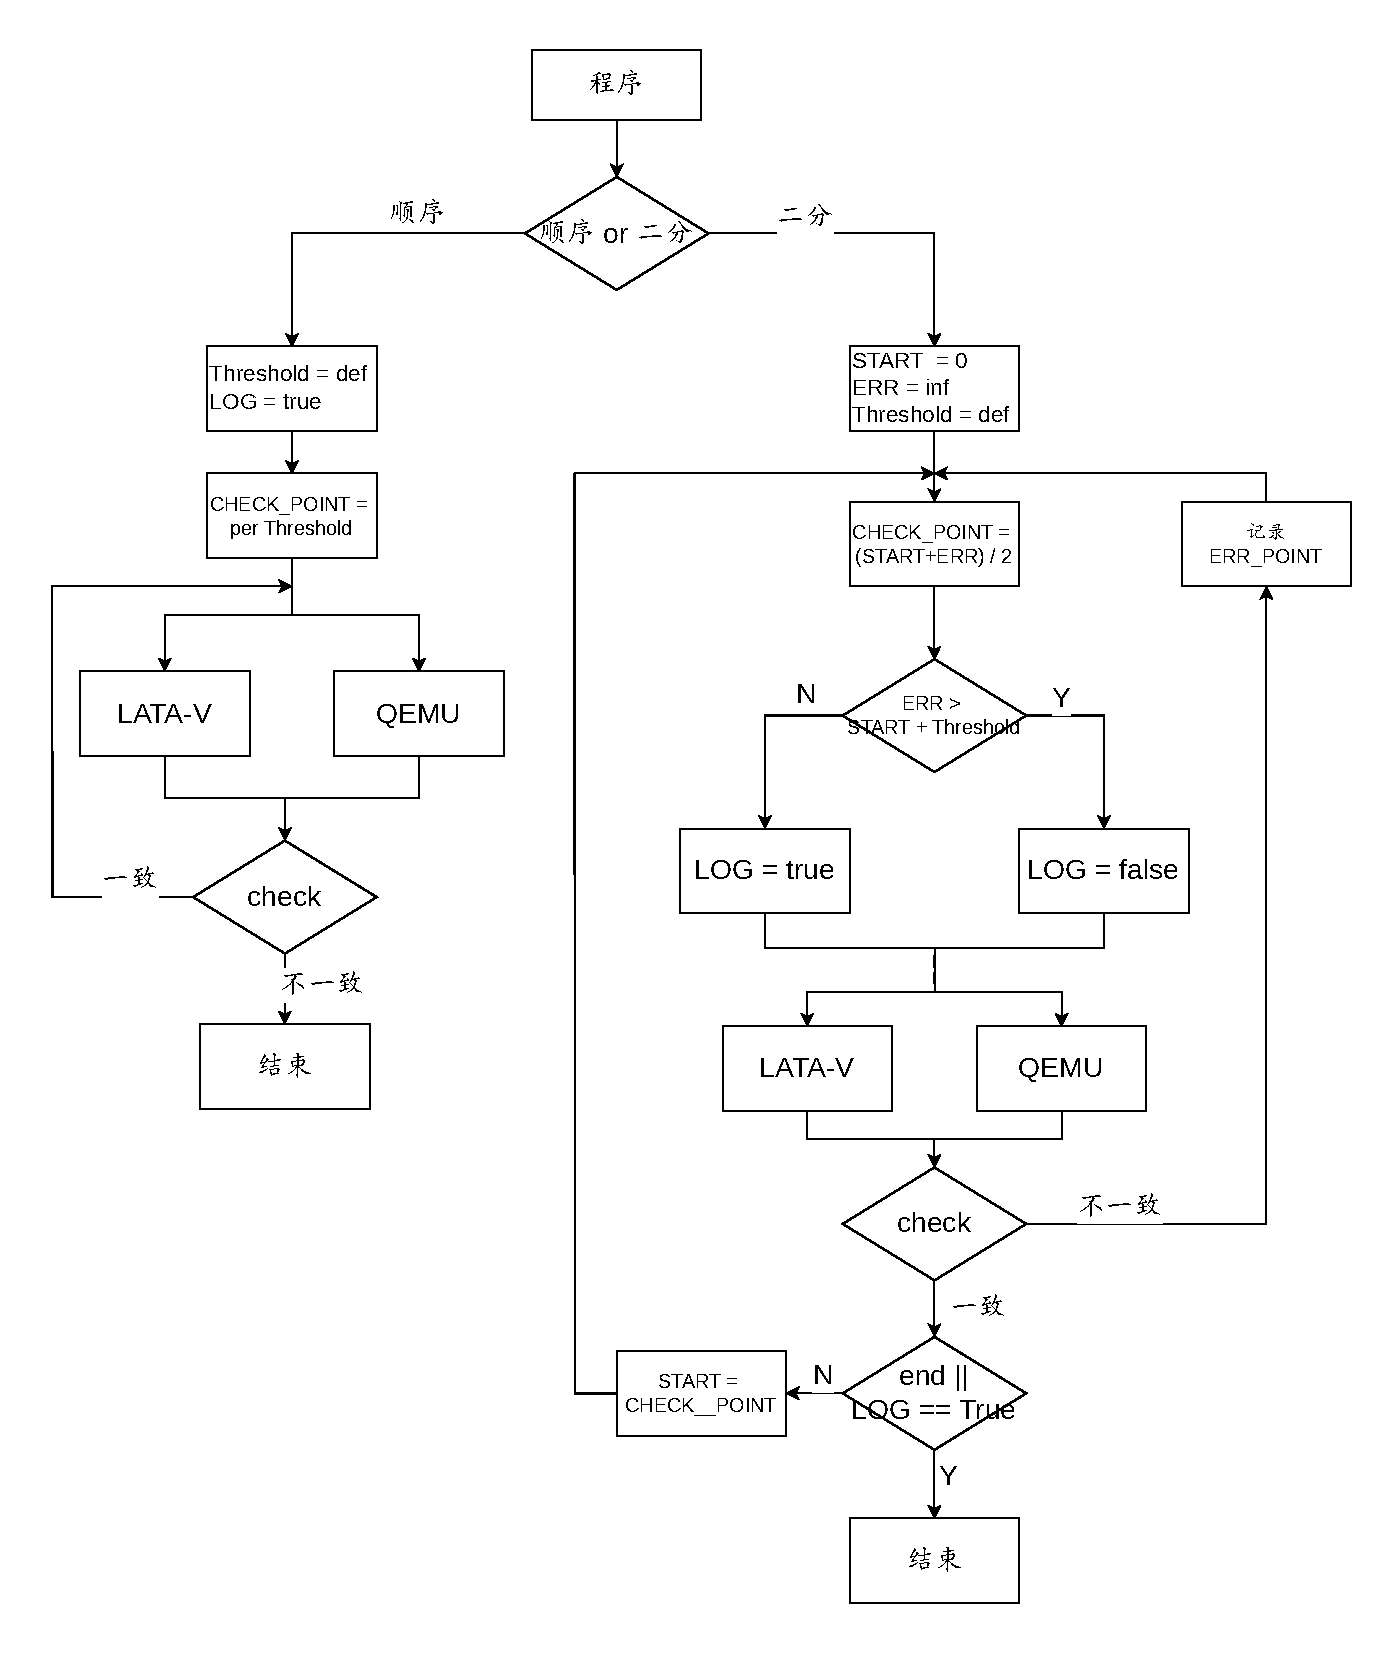
\includegraphics[width=1\textwidth]{QEMU_LATA-V}
    \bicaption{\enspace 基于QEMU的调试框架}{\enspace Debugging framework based on QEMU}
    \label{fig:QEMU_LATA-V}
\end{figure}

\subsection{LATA-V的瓶颈分析}
LATA-V的瓶颈分析是在指令膨胀率的基础上完成的。在SPEC CPU 2006的负载上,统计LATA-V的动态指令数频率,如图\ref{fig:arm64operands_combined}所示。膨胀率分析会在动态指令数占比和单指令的膨胀的基础上,计算得出某类指令在总体膨胀中的占比;单指令膨胀和总体的膨胀数据还未统计完成。

% \subsubsection{LATA-V的指令膨胀率分析}    
% \subsubsection{基于指令膨胀率的瓶颈分析}
\begin{figure}[!htbp]
    \centering
    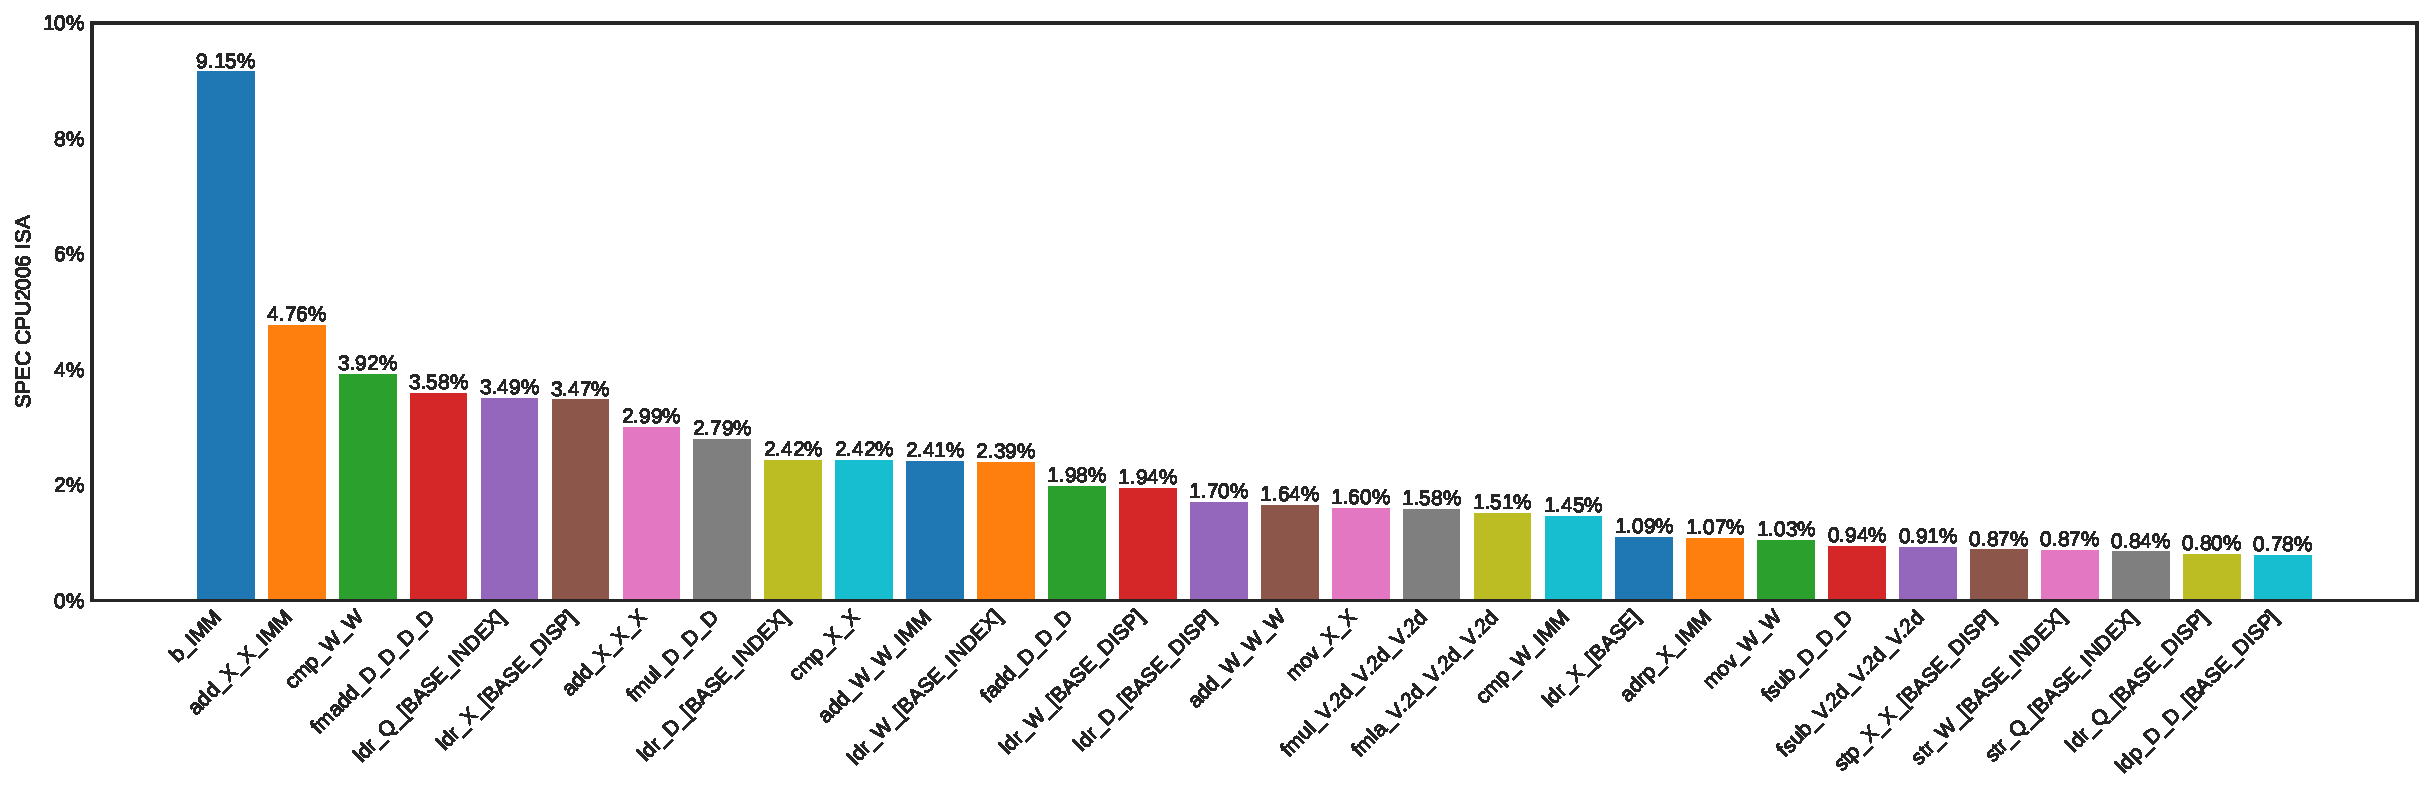
\includegraphics[width=1\textwidth]{arm64operands_combined}
    \bicaption{\enspace SPEC CPU 2006动态指令数占比}{\enspace Proportion of Dynamic Instruction Count in SPEC CPU 2006}
    \label{fig:arm64operands_combined}
\end{figure}
\subsection{LATA-V的性能优化}
% \subsubsection{基础的指令优化}
\subsubsection{复用X86-LBT优化}
% 二进制翻译是一种可以实现指令集模拟的技术,通常需要做到对指令集语义的精确模拟,其中也包括对标志位的模拟。在一个显式标志位运算的架构中,有两种方案可以实现对标志位的模拟。一种是纯软件的模拟,翻译器可以整合多条比较指令的结果实现对标志位的模拟;但是这种软件上的模拟开销比较大,单是一个标志位就需要多条指令进行模拟,对于标志位较多的架构(例如X86架构6个标志位),可能需要20-30条指令模拟一条运算指令。另一种模拟的方案则是基于硬件拓展的方式,在显式运算的架构中实现一个拓展的标志位寄存器和相应架的构标志位运算指令;通过这种软硬结合的方式,翻译器能够以较少的指令完成一条指令的模拟;同时拓展指令只会被用在翻译器中,没有指令集兼容的负担。
复用X86-LBT优化的主要思想是将龙芯平台已经实现的X86硬件拓展指令用在ARM标志位运算指令的翻译中,而想要达成指令的复用,要求X86和ARM平台的标志位和指令对标志位的影响有相似性。

X86架构有一套丰富的状态标志位,存储在标志寄存器(EFLAGS)中。这些标志位包括进位标志(CF)、奇偶标志(PF)、辅助标志(AF)、零标志(ZF)、符号标志(SF)、溢出标志(OF),在EFLAGS寄存器中的位置如图\ref{fig:eflag}a所示;
ARM 处理器的状态寄存器(FPSCR)中有 4 位标志位(NZCV),分别对应符号标志(N)、零标志(Z)、进位标志(C)和溢出标志(V),在FPSCR寄存器中的位置如图\ref{fig:eflag} b所示;其中ARM中的标志位N,Z,C,V分别对应x86中的标志位SF,ZF,CF和OF。
分析了2种架构标志位的设计不难发现,且相比于x86架构,ARM架构的标志位恰好是x86的子集,也就是说只要实现了X86的标志位寄存器,就统一了2种架构的标志位寄存器,唯一需要调整的是标志位在各自状态寄存器中的位置。
\begin{figure}[!htbp]
    \centering
    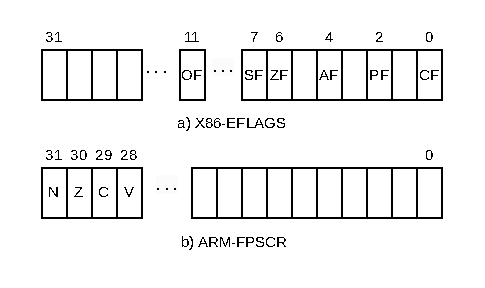
\includegraphics[width=0.7\textwidth]{eflag}
    \bicaption{\enspace x86和ARM运算标志位}{\enspace Arithmetic Flags of x86 and ARM}
    \label{fig:eflag}
\end{figure}

% \begin{table}[!htbp]
%     \bicaption{\enspace 指令对标志位的影响}{\enspace The impact of instructions on flag bits}
%     \label{tab:flag_effect}
%     \centering
%     \footnotesize % 设置字体大小
%     \setlength{\tabcolsep}{4pt} % 设置列间距
%     \renewcommand{\arraystretch}{1.2} % 设置行距
%     \begin{tabular}{l c}
%         \hline
%         \textbf{缩写} & \textbf{含义} \\ 
%         \hline
%         T & Tests,使用该标志位 \\ 
%         M & Modify,置0或者置1 \\ 
%         0 & Reset,置0 \\ 
%         1 & Set,置1 \\ 
%         --- & Undefined,未定义 \\ 
%         R & Restore,恢复之前的值 \\ 
%         Blank & 空表示不影响 \\ 
%         \hline
%     \end{tabular}
% \end{table}

指令对标志位的影响如表\ref{tab:flag_effect}所示:其中表\ref{tab:flag_effect}a定义了7种指令对标志位的影响,表\ref{tab:flag_effect}b和表\ref{tab:flag_effect}c分别表示ARM指令和x86指令标志位的影响。
从表\ref{tab:flag_effect}中可以看出,x86架构中几乎所有的算术、逻辑和移位运算指令都会影响ELFAGS寄存器,并且x86架构存在子寄存器运算的情况,包括8位,16位,32位和64位的寄存器长度;
ARM架构中只有部分的运算和逻辑指令会影响FPSCR寄存器,移位指令本身并不影响标志位,同时ARM中的寄存器长度只有32位和64位;
所以,从指令种类的角度来说,大部分ARM的标志位运算指令能在x86中找到对应逻辑的指令。

经过测试可以发现,ARM中的ADCS,ADDS,ANDS,EORS,CMP指令对标志位的修改和x86中的ADC,ADD,AND,XOR和SUB指令的行为一致。BICS指令本身的语义比较复杂,但是最终会影响标志位的是两个操作数的与操作,所以只需要在执行BICS执行之前正确维护操作数的值即可;SBCS和CMN指令的语义都是先将减数按位取反,不同的是SBCS保持进位不变,CMN指令会将进位临时置1,最终影响标志位的是被减数、减数取反后的数以及进位三者相加的结果,所以SBCS和CMN指令对标志位的影响可以复用x86的ADC指令。

\vspace{5cm}
\begin{table}[!htbp]
    \bicaption{\enspace 指令对标志位的影响}{\enspace The impact of instructions on flag bits}
    \label{tab:flag_effect}
    \centering
    \footnotesize % 设置字体大小
    \setlength{\tabcolsep}{4pt} % 设置列间距
    \renewcommand{\arraystretch}{1.2} % 设置行距
    
    \begin{minipage}{0.4\textwidth} % 左侧 minipage,占40%
        \centering
        \textbf{a) 指令影响标志位的说明} \\
        \vspace{0.2cm}
        \begin{tabular}{l c}
            \hline
            \textbf{缩写} & \textbf{含义} \\ 
            \hline
            T & Tests,使用该标志位 \\ 
            M & Modify,置0或者置1 \\ 
            0 & Reset,置0 \\ 
            1 & Set,置1 \\ 
            --- & Undefined,未定义 \\ 
            R & Restore,恢复之前的值 \\ 
            Blank & 空表示不影响 \\ 
            \hline
        \end{tabular}
        
        \vspace{0.5cm} % 控制 a 和 c 之间的间距
        
        \textbf{b) ARM指令对标志位的影响} \\
        \vspace{0.2cm}
        \begin{tabular}{lcccc}
            \hline
            Instructions & N & Z & C & V \\
            \hline
            01.ADCS & M & M & M & TM \\
            02.ADDS & M & M & M & M \\
            03.ANDS & M & M & 0 & 0 \\
            04.BICS & M & M & 0 & 0 \\
            05.EORS & M & M & M & M \\
            06.CMP & M & M & M & M \\
            07.CMN & M & M & M & M \\
            08.SBCS & M & M & M & TM \\
            \hline
        \end{tabular}
    \end{minipage}%
    \hfill % 控制左右间距
    \begin{minipage}{0.6\textwidth} % 右侧 b,占60%
        \centering
        \textbf{c) X86指令对标志位的影响} \\
        \vspace{0.2cm} % 调整表头与表格之间的距离
        \begin{tabular}{lcccccc}
            \hline
            Instructions & OF & SF & ZF & AF & PF & CF \\
            \hline
            01.ADC & M & M & M & M & M & TM \\
            02.ADD & M & M & M & M & M & M \\
            03.AND & 0 & M & M & --- & M & 0 \\
            04.CMP & M & M & M & M & M & M \\
            05.DEC & M & M & M & M & M &  \\
            06.IMUL & M & --- & --- & --- & --- & M \\
            07.MUL & M & --- & --- & --- & --- & M \\
            08.NEG & M & M & M & M & M & M \\
            09.OR & 0 & M & M & --- & M & 0 \\
            10.ROL/ROR & M &  &  &  &  & M \\
            12.SAL/SAR/SHL/SHR & M & M & M & --- & M & M \\
            16.SBB & M & M & M & M & M & TM \\
            \hline
        \end{tabular}
    \end{minipage}
\end{table}

% \vspace{1cm}
% \begin{table}[!htbp]
%     \caption{\enspace 影响X86和ARM标志位的指令}{\enspace Instructions Affecting X86 and ARM Flags}
%     \label{tab:x86_arm_flags}
%     \centering
%     \footnotesize% fontsize
%     \setlength{\tabcolsep}{4pt}% column separation
%     \renewcommand{\arraystretch}{1.2}% row space 
    
%     \begin{minipage}{0.45\textwidth}
%         \centering
%         \vspace{0.5cm} % 调整表头与表格之间的距离
%         \textbf{a) X86} \\
%         \vspace{0.1cm} % 调整表头与表格之间的距离
%         \begin{tabular}{lcccccc}
%             \hline
%             Instructions & OF & SF & ZF & AF & PF & CF \\
%             \hline
%             01.ADC & M & M & M & M & M & TM \\
%             02.ADD & M & M & M & M & M & M \\
%             03.AND & 0 & M & M & --- & M & 0 \\
%             04.CMP & M & M & M & M & M & M \\
%             05.DEC & M & M & M & M & M &  \\
%             06.IMUL & M & --- & --- & --- & --- & M \\
%             07.MUL & M & --- & --- & --- & --- & M \\
%             08.NEG & M & M & M & M & M & M \\
%             09.OR & 0 & M & M & --- & M & 0 \\
%             10.ROL/ROR & M &  &  &  &  & M \\
%             12.SAL/SAR/SHL/SHR & M & M & M & --- & M & M \\
%             16.SBB & M & M & M & M & M & TM \\
%             \hline
%         \end{tabular}
%     \end{minipage}
%     \hspace{1cm} % 添加水平间距
%     \begin{minipage}{0.45\textwidth}
%         \centering
%         \textbf{b) ARM} \\
%         \vspace{0.1cm} % 调整表头与表格之间的距离
%         \begin{tabular}{lcccc}
%             \hline
%             Instructions & N & Z & C & V \\
%             \hline
%             01.ADCS & M & M & M & TM \\
%             02.ADDS & M & M & M & M \\
%             03.ANDS & M & M & 0 & 0 \\
%             04.BICS & M & M & 0 & 0 \\
%             05.EORS & M & M & M & M \\
%             06.CMP & M & M & M & M \\
%             07.CMN & M & M & M & M \\
%             08.SBCS & M & M & M & TM \\
%             \hline
%         \end{tabular}
%     \end{minipage}
% \end{table}

% \begin{figure}[!htbp]
%     \centering
%     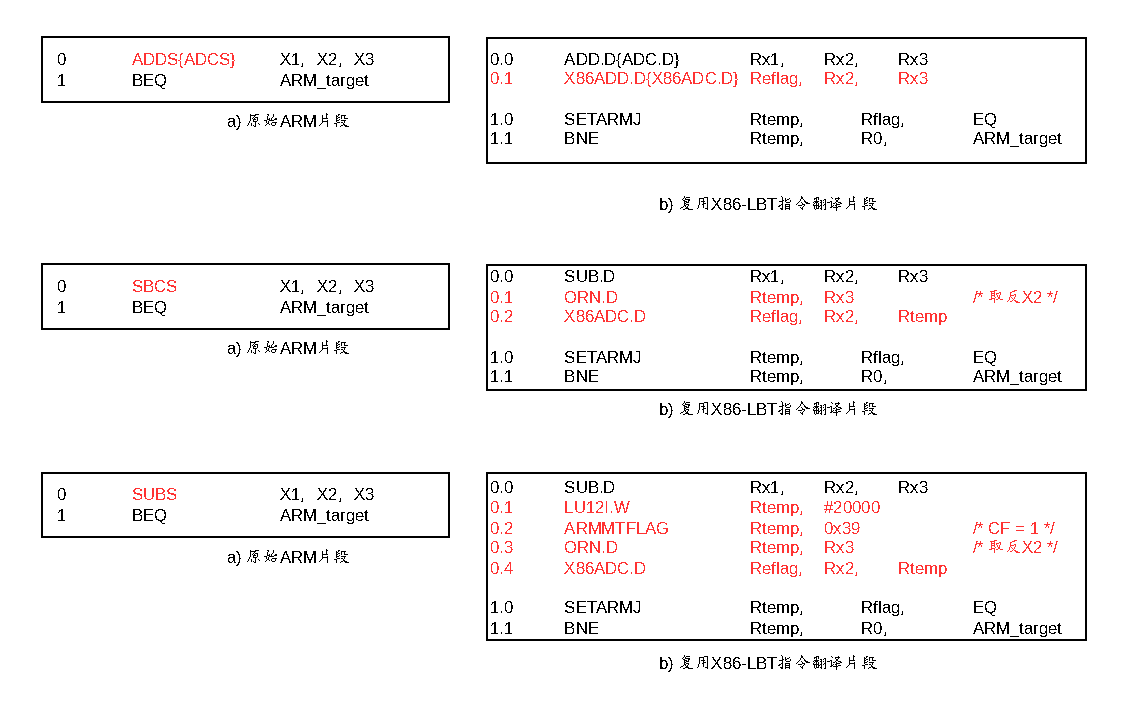
\includegraphics[width=1\textwidth]{LBT-X86_Optimization}
%     \bicaption{\enspace x86和ARM的运算标志位}{\enspace }
%     \label{fig:LBT-X86_Optimization}
% \end{figure}

\subsubsection{高位清零消除优化}
在 ARM64 中,写 32 位子寄存器会被零拓展到 64 位;在 LoongArch 中,写 32 位子寄存器会被符号拓展成 64 位。在翻译 ARM64 的 32 位子寄存器运算时,需要额外的指令实现零拓展。

优化主要分为两部分:
\begin{itemize}
    \item \textbf{基本块内的优化}:对寄存器的操作可以分为 4 类:\texttt{Read\_w},\texttt{Write\_w},\texttt{Read\_x},\texttt{Write\_x},分别表示对 32 位/64 位寄存器的读写;分析每个寄存器的数据流,只有出现先 \texttt{Write\_w} 后 \texttt{Read\_x} 的数据流时,才需要在 \texttt{Read\_x} 前对高位寄存器清零。同时在每个基本块尾部,需要对数据流中最后存在 \texttt{Write\_w} 操作的寄存器进行高位清零。
    \item \textbf{基本块间的优化}:由于每个基本块只有两个出口,对于存在循环的基本块,在基本块的尾部的清零操作可以移动到基本块出口,减少当前循环的指令数量。
\end{itemize}

\begin{figure}[!htbp]
    \centering
    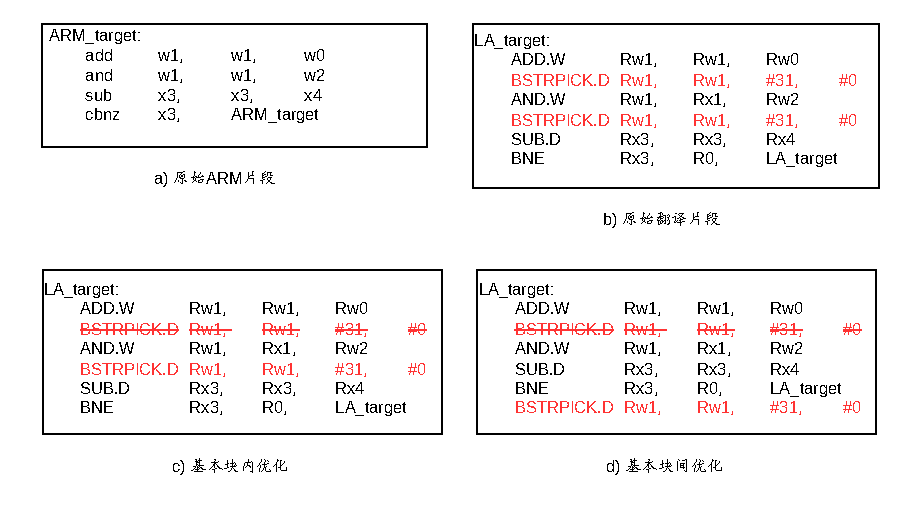
\includegraphics[width=1\textwidth]{High-bit_Zeroing_Elimination_Optimization}
    \bicaption{\enspace 高位清零消除优化}{\enspace High-bit Zeroing Elimination Optimization}
    \label{fig:High-bit_Zeroing_Elimination_Optimization}
\end{figure}

\section{下一步工作计划和内容,预计答辩时间}
\subsection*{2024 年 2 月-2024 年 3 月}
\begin{itemize}[left=0pt]
    \item 完善程序静态特征提取的 PASS,目标是提取到 55 个相关的静态特征;
    \item 以 Csmith 生成 10000 个随机 C 语言程序,以迭代优化得到的优化配置选项进行数据标注,配置程序静态特征提取,构建训练数据集;
    \item 完成人工神经网络的训练,集成到 GCC 编译器插件中;
    \item 进行机器学习模型化预测部分的有效性验证。
\end{itemize}

\subsection*{2024 年 3 月-2024 年 4 月}
\begin{itemize}[left=0pt]
    \item 完善整体架构集成化测试和有效性验证;
    \item 设计参数相关实验收集更细粒度的实验数据;
    \item 撰写毕业论文。
\end{itemize}

\section{已取得科研成果列表(已发表、待发表学术论文、专利等)}
无
\citestyle{numbers}
\nocite{*}% 使文献列表显示所有参考文献(包括未引用文献)
%---------------------------------------------------------------------------%
